
%%%%%%%%%%%%%%%%%%%%%%%%%%%%%%%%%%%%%%%%%%%%%%%%%%%%%%%%%%%%%%%%%%%%%%%%%%%%%%%%%%
\begin{frame}[fragile]\frametitle{}
\begin{center}
{\Large Generic Applications of Prompts}
\end{center}
\end{frame}

%%%%%%%%%%%%%%%%%%%%%%%%%%%%%%%%%%%%%%%%%%%%%%%%%%%%%%%%%%%
\begin{frame}[fragile]\frametitle{Text Generation}

\begin{center}
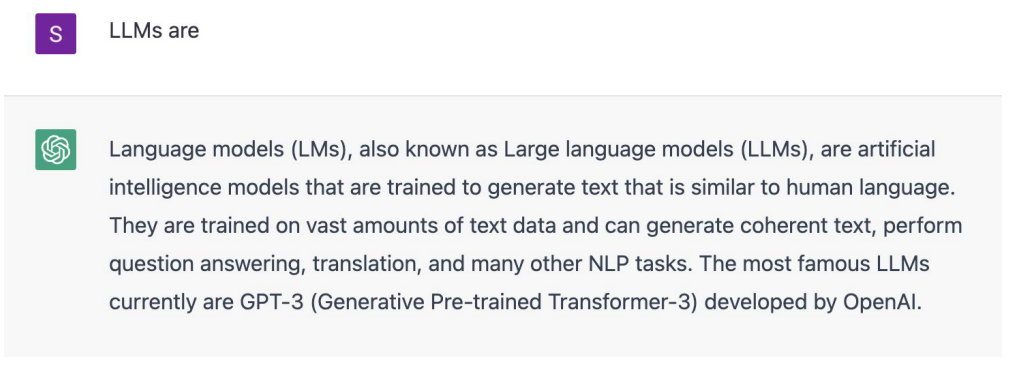
\includegraphics[width=\linewidth,keepaspectratio]{promptengg10}

{\tiny (Ref: Prompt Engineering Sudalai Rajkumar)}

\end{center}		
		


\end{frame}

%%%%%%%%%%%%%%%%%%%%%%%%%%%%%%%%%%%%%%%%%%%%%%%%%%%%%%%%%%%
\begin{frame}[fragile]\frametitle{Text Classification}

\begin{center}
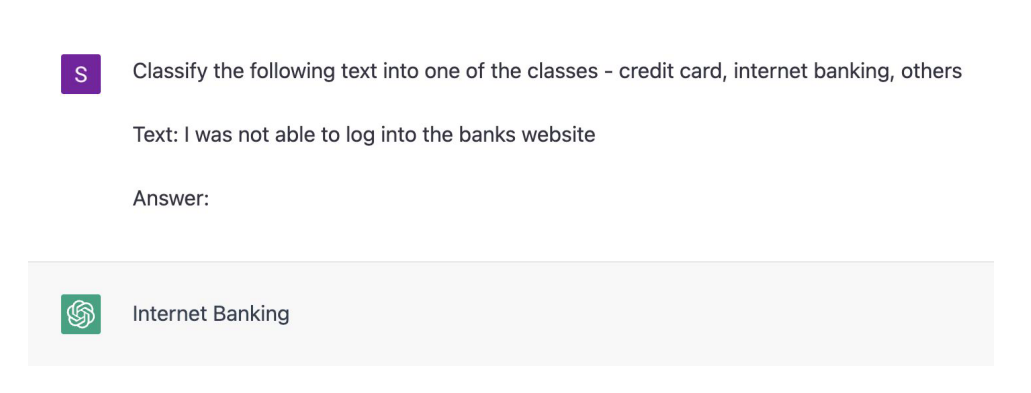
\includegraphics[width=\linewidth,keepaspectratio]{promptengg11}

{\tiny (Ref: Prompt Engineering Sudalai Rajkumar)}

\end{center}		
		


\end{frame}

%%%%%%%%%%%%%%%%%%%%%%%%%%%%%%%%%%%%%%%%%%%%%%%%%%%%%%%%%%%
\begin{frame}[fragile]\frametitle{Text Translation}

\begin{center}

\includegraphics[width=\linewidth,keepaspectratio]{promptengg12}

{\tiny (Ref: Prompt Engineering Sudalai Rajkumar)}

\end{center}		
		


\end{frame}

%%%%%%%%%%%%%%%%%%%%%%%%%%%%%%%%%%%%%%%%%%%%%%%%%%%%%%%%%%%
\begin{frame}[fragile]\frametitle{Text Comprehension}

\begin{center}
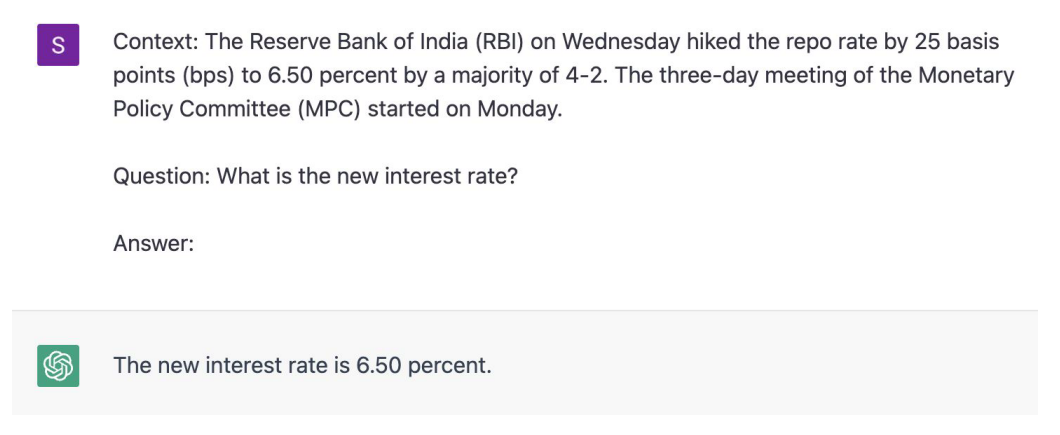
\includegraphics[width=\linewidth,keepaspectratio]{promptengg13}

{\tiny (Ref: Prompt Engineering Sudalai Rajkumar)}

\end{center}		
		


\end{frame}

%%%%%%%%%%%%%%%%%%%%%%%%%%%%%%%%%%%%%%%%%%%%%%%%%%%%%%%%%%%
\begin{frame}[fragile]\frametitle{Text Summarization}

\begin{center}

\includegraphics[width=\linewidth,keepaspectratio]{promptengg14}

{\tiny (Ref: Prompt Engineering Sudalai Rajkumar)}

\end{center}		
		


\end{frame}


%%%%%%%%%%%%%%%%%%%%%%%%%%%%%%%%%%%%%%%%%%%%%%%%%%%%%%%%%%%
\begin{frame}[fragile]\frametitle{Question Answering}

\begin{center}
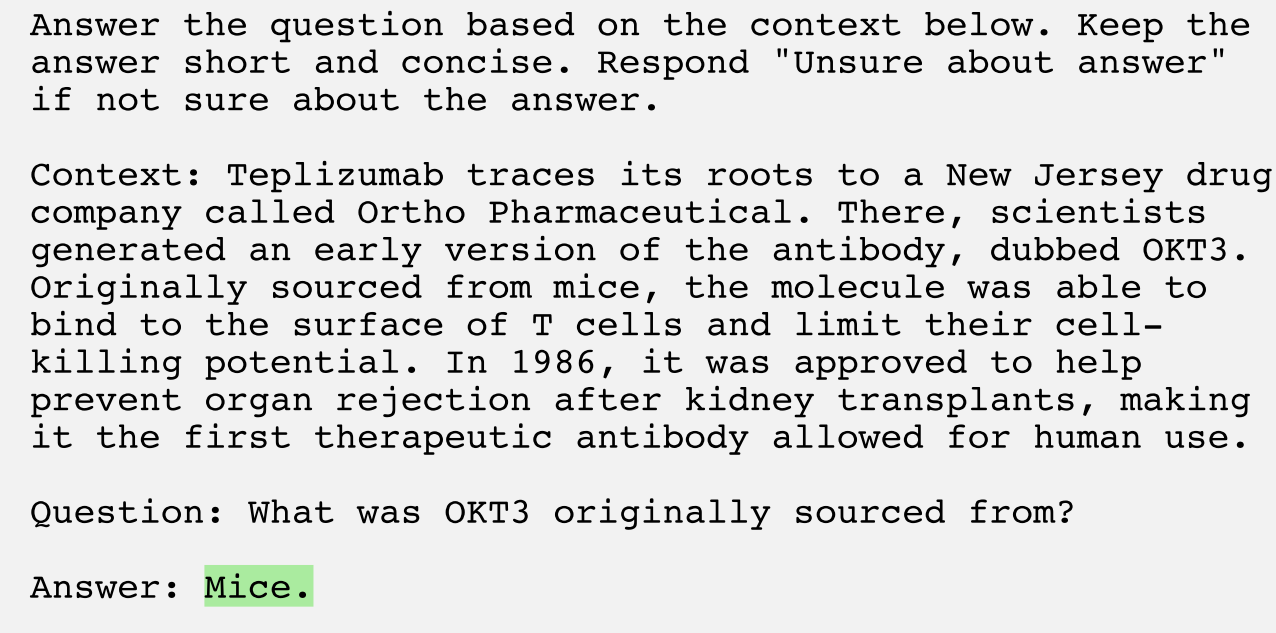
\includegraphics[width=\linewidth,keepaspectratio]{promptengg43}

{\tiny (Ref: Prompt Engineering A lecture by DAIR.AI)}

\end{center}
\end{frame}


%%%%%%%%%%%%%%%%%%%%%%%%%%%%%%%%%%%%%%%%%%%%%%%%%%%%%%%%%%%
\begin{frame}[fragile]\frametitle{Role Playing}

\begin{center}
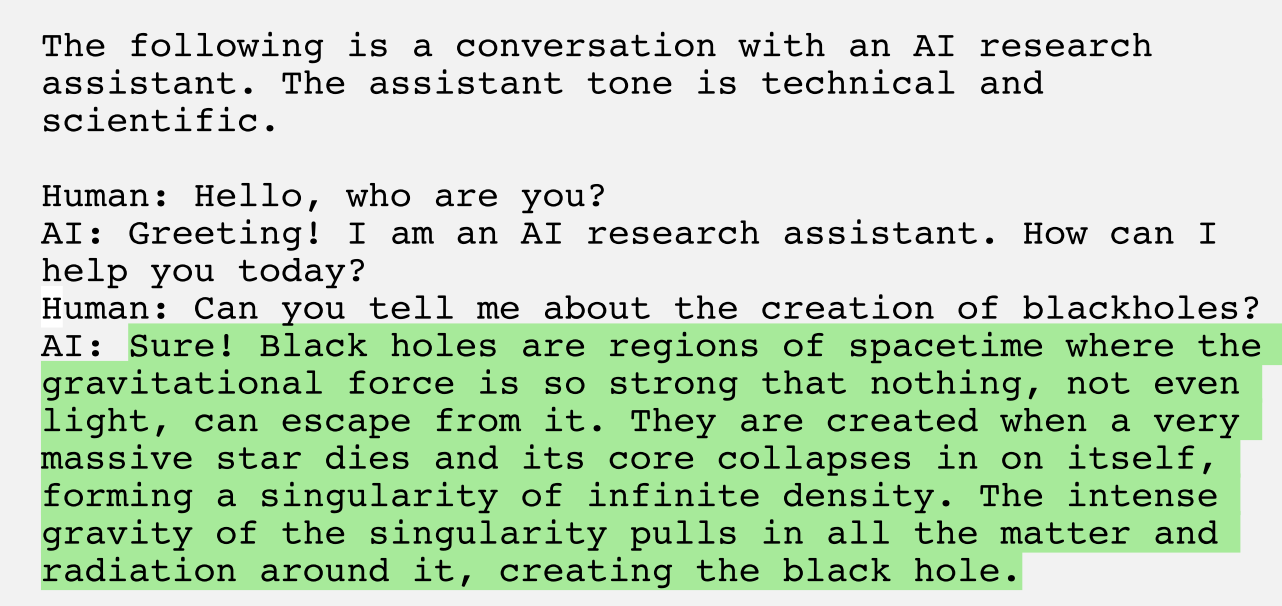
\includegraphics[width=\linewidth,keepaspectratio]{promptengg44}

{\tiny (Ref: Prompt Engineering A lecture by DAIR.AI)}

\end{center}
\end{frame}


%%%%%%%%%%%%%%%%%%%%%%%%%%%%%%%%%%%%%%%%%%%%%%%%%%%%%%%%%%%
\begin{frame}[fragile]\frametitle{Image Generation}

\begin{center}
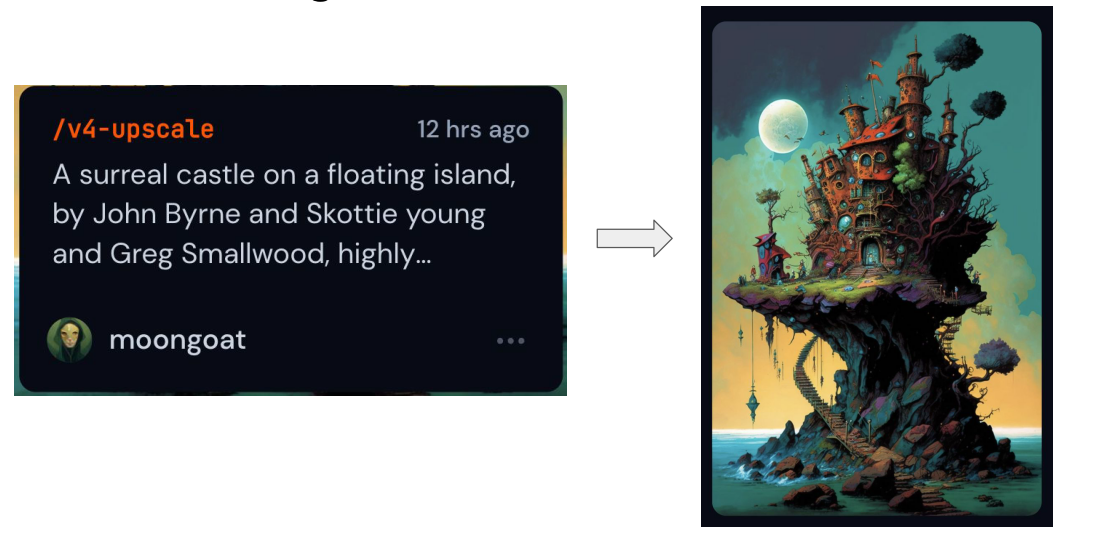
\includegraphics[width=\linewidth,keepaspectratio]{promptengg15}

{\tiny (Ref: Prompt Engineering Sudalai Rajkumar)}

\end{center}		
		
		
Models / Tools: Dall-E , Midjourney, Stable Diffusion

\end{frame}

%%%%%%%%%%%%%%%%%%%%%%%%%%%%%%%%%%%%%%%%%%%%%%%%%%%%%%%%%%%
\begin{frame}[fragile]\frametitle{Prompting Midjourney}


\begin{columns}
    \begin{column}[T]{0.6\linewidth}
		\begin{center}
		
\includegraphics[width=\linewidth,keepaspectratio]{promptengg67}

		{\tiny (Ref: The Complete Prompt Engineering for AI Bootcamp (2023))}
		\end{center}	
    \end{column}
    \begin{column}[T]{0.4\linewidth}
		This is a simple prompt we can use with Midjourney when generating a stock photo of a business meeting.
    \end{column}
  \end{columns}
\end{frame}

%%%%%%%%%%%%%%%%%%%%%%%%%%%%%%%%%%%%%%%%%%%%%%%%%%%%%%%%%%%
\begin{frame}[fragile]\frametitle{Providing Examples to Midjourney}


\begin{columns}
    \begin{column}[T]{0.6\linewidth}
		\begin{center}
		
\includegraphics[width=\linewidth,keepaspectratio]{promptengg68}

		{\tiny (Ref: The Complete Prompt Engineering for AI Bootcamp (2023))}
		\end{center}	
    \end{column}
    \begin{column}[T]{0.4\linewidth}
		Providing examples in your prompts improves the reliability of your output.
		Transform the base image with the words in the prompt to make it your own.
    \end{column}
  \end{columns}
\end{frame}

%%%%%%%%%%%%%%%%%%%%%%%%%%%%%%%%%%%%%%%%%%%%%%%%%%%%%%%%%%%
\begin{frame}[fragile]\frametitle{Giving Direction to Midjourney}


\begin{columns}
    \begin{column}[T]{0.6\linewidth}
		\begin{center}
		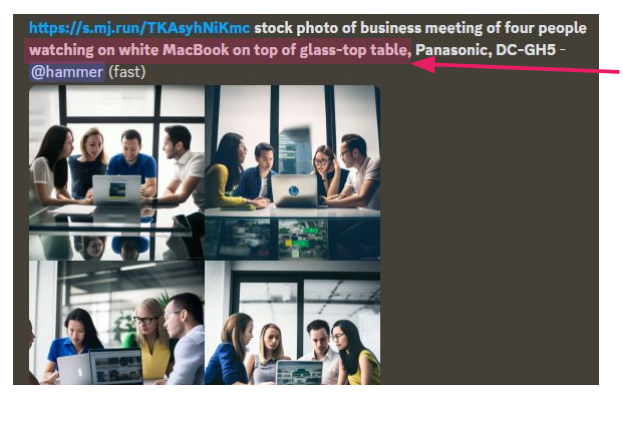
\includegraphics[width=\linewidth,keepaspectratio]{promptengg70}

		{\tiny (Ref: The Complete Prompt Engineering for AI Bootcamp (2023))}
		\end{center}	
    \end{column}
    \begin{column}[T]{0.4\linewidth}
		Describing what you’re imagining, gets you output that matches your vision.
		Transform the base image with the words in the prompt to make it your own.
    \end{column}
  \end{columns}
\end{frame}

%%%%%%%%%%%%%%%%%%%%%%%%%%%%%%%%%%%%%%%%%%%%%%%%%%%%%%%%%%%
\begin{frame}[fragile]\frametitle{Formatting Responses to Midjourney}


\begin{columns}
    \begin{column}[T]{0.6\linewidth}
		\begin{center}
		
\includegraphics[width=\linewidth,keepaspectratio]{promptengg72}

		{\tiny (Ref: The Complete Prompt Engineering for AI Bootcamp (2023))}
		\end{center}	
    \end{column}
    \begin{column}[T]{0.4\linewidth}
		Demonstrating your required response format, minimizes time spent parsing errors. 
		Use formats that are well-recognized and likely to appear in training data.
    \end{column}
  \end{columns}
\end{frame}

%%%%%%%%%%%%%%%%%%%%%%%%%%%%%%%%%%%%%%%%%%%%%%%%%%%%%%%%%%%
\begin{frame}[fragile]\frametitle{Evaluating Quality to Midjourney}


\begin{columns}
    \begin{column}[T]{0.6\linewidth}
		\begin{center}
		
\includegraphics[width=\linewidth,keepaspectratio]{promptengg74}

		{\tiny (Ref: The Complete Prompt Engineering for AI Bootcamp (2023))}
		\end{center}	
    \end{column}
    \begin{column}[T]{0.4\linewidth}
		Test prompts to iterate and improve on the reliability of your results.
		Try different combinations systematically to identify where it fails and succeeds.
    \end{column}
  \end{columns}
\end{frame}

%%%%%%%%%%%%%%%%%%%%%%%%%%%%%%%%%%%%%%%%%%%%%%%%%%%%%%%%%%%
\begin{frame}[fragile]\frametitle{Chaining AIs to Midjourney}


\begin{columns}
    \begin{column}[T]{0.6\linewidth}
		\begin{center}
		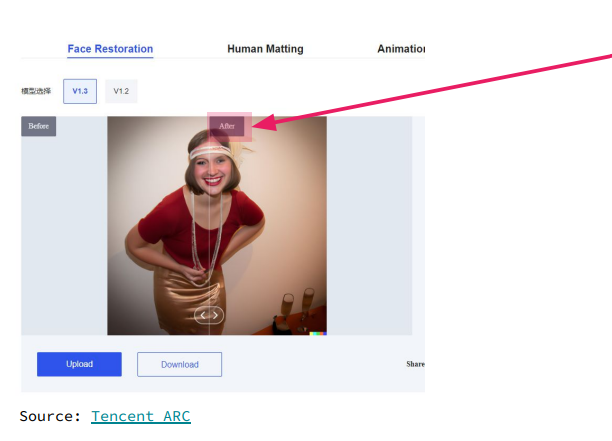
\includegraphics[width=\linewidth,keepaspectratio]{promptengg76}

		{\tiny (Ref: The Complete Prompt Engineering for AI Bootcamp (2023))}
		\end{center}	
    \end{column}
    \begin{column}[T]{0.4\linewidth}
		Combine multiple AI responses, allows you to complete more complex tasks.
		Special-purpose AIs can serve well for common tasks, and correct the mistakes of general models.
    \end{column}
  \end{columns}
\end{frame}

%%%%%%%%%%%%%%%%%%%%%%%%%%%%%%%%%%%%%%%%%%%%%%%%%%%%%%%%%%%
\begin{frame}[fragile]\frametitle{Code Generation}

\begin{center}
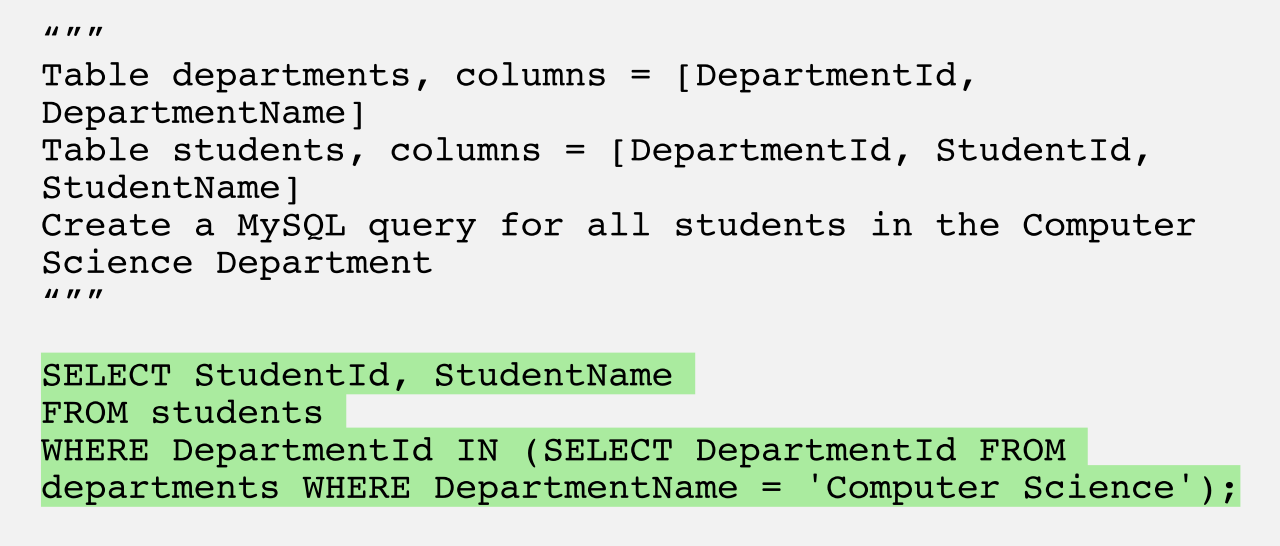
\includegraphics[width=\linewidth,keepaspectratio]{promptengg45}

{\tiny (Ref: Prompt Engineering A lecture by DAIR.AI)}

\end{center}
\end{frame}

%%%%%%%%%%%%%%%%%%%%%%%%%%%%%%%%%%%%%%%%%%%%%%%%%%%%%%%%%%%
\begin{frame}[fragile]\frametitle{Reasoning}

\begin{center}
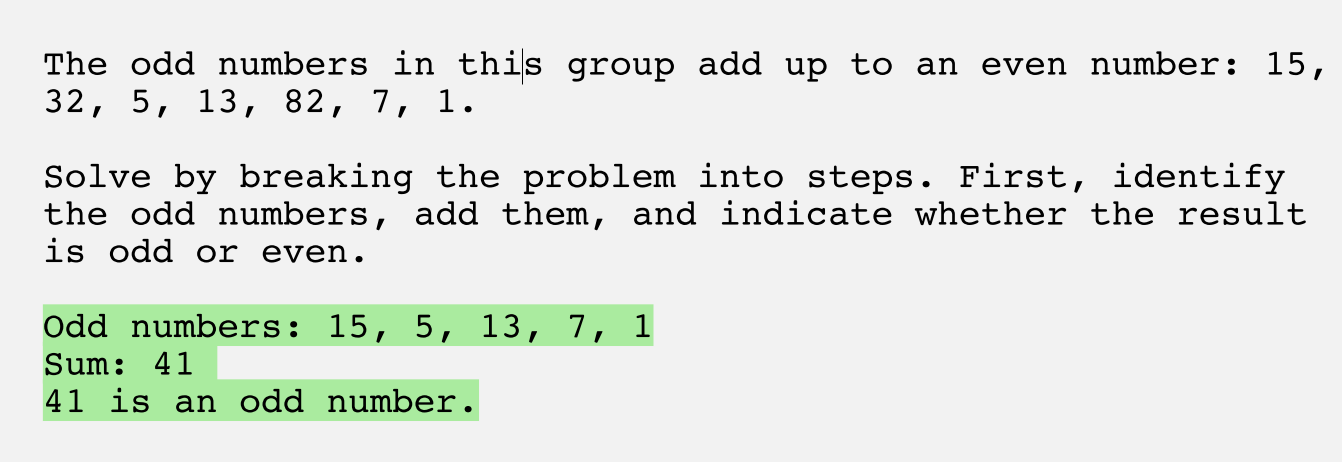
\includegraphics[width=\linewidth,keepaspectratio]{promptengg46}

{\tiny (Ref: Prompt Engineering A lecture by DAIR.AI)}

\end{center}
\end{frame}




%%%%%%%%%%%%%%%%%%%%%%%%%%%%%%%%%%%%%%%%%%%%%%%%%%%%%%%%%%%
\begin{frame}[fragile]\frametitle{For generating code using Codex}

Provide Codex with a prompt consisting of the following:



\begin{itemize}
\item  High level task description: Tell the model to use a helpful tone when outputting natural language
\item  High level context: Describe background information like API hints and database schema to help the model understand the task
\item  Examples: Show the model examples of what you want
\item  User input: Remind the model what the user has said before
\end{itemize}	 

{\tiny (Ref: https://microsoft.github.io/prompt-engineering/)}

\end{frame}

% %%%%%%%%%%%%%%%%%%%%%%%%%%%%%%%%%%%%%%%%%%%%%%%%%%%%%%%%%%%
% \begin{frame}[fragile]\frametitle{For Cypher code For Neo4j}


% Provide examples within prompt:

% {\tiny (Ref:https://github.com/tomasonjo/langchain2neo4j)}

% \begin{lstlisting}
% # Who played in Top Gun?
% MATCH (m:Movie)<-[r:ACTED_IN]-(a)
% RETURN {{actor: a.name, role: r.role}} AS result
% # What is the plot of the Copycat movie?
% MATCH (m:Movie {{title: "Copycat"}})
% RETURN {{plot: m.plot}} AS result
% # Did Luis Guzman appear in any other movies?
% MATCH (p:Person {{name:"Luis Guzman"}})-[r:ACTED_IN]->(movie)
% RETURN {{movie: movie.title, role: r.role}} AS result
% # Do you know of any matrix movies?
% MATCH (m:Movie)
% WHERE toLower(m.title) CONTAINS toLower("matrix")
% RETURN {{movie:m.title}} AS result
% \end{lstlisting}	 


% \end{frame}

% %%%%%%%%%%%%%%%%%%%%%%%%%%%%%%%%%%%%%%%%%%%%%%%%%%%%%%%%%%%
% \begin{frame}[fragile]\frametitle{Crazy ideas}

% \begin{itemize}
% \item Stop asking ChatGPT for information - start an actual conversation.
% “What's the population of Topeka?” Gah! ChatGPT isn't Google. Google is Google. ChatGPT is a brilliant, patient thought partner.
% EXAMPLE: Tell it *why* you want to know about Topeka. “I'm starting a consulting business in Topeka, I have \$20k, two kids in middle school, I studied biology, I worked for McKinsey. What are ten reasons my business might succeed or fail?”
% Feed it more and more detail about your work experience, family, etc. - that's where the magic happens.

% \item Create actual characters to debate your Big Idea before presenting it.
% Test your work ideas on ChatGPT, which will play the roles of colleagues.
% EXAMPLE: Tell ChatGPT “Play 4 roles for me: Be my company's CEO, CMO, CTO, and CFO. (Describe each person- Technical? Fiscally conservative? Passive aggressive?) Probe the following idea for weaknesses.”
% A bit traumatic, right? Okay, Step Two: Tell ChatGPT “Now become a smarter version of all those executives and give counter-arguments as to why my idea is brilliant.”
% Invite historical guests! Ask Steve Jobs to make a case for your idea! Or Einstein!

% \end{itemize}	 

% {\tiny (Ref: LinkedIn post by Dr Joerg Storm)}
			

% \end{frame}

% %%%%%%%%%%%%%%%%%%%%%%%%%%%%%%%%%%%%%%%%%%%%%%%%%%%%%%%%%%%
% \begin{frame}[fragile]\frametitle{Crazy ideas}

% \begin{itemize}

% \item ChatGPT is built for creatives. And it wants ALL the smoke.
% ChatGPT isn't a racehorse - it's freakin' Seabiscuit. It wants to show off. People give up because they pose a general question and get a general answer. Get specific!
% EXAMPLE:
% Don't ask “What are strategies for handling an annoying co-worker?”
% Instead, try “I work in a San Jose crayon factory in quality control. My colleague points out every crayon I've missed and asks gas-lighting questions. What are three indirect ways to stop his behavior and what is one direct thing I can say?” Ask follow up questions.

% \item Talk to it like a trusted, brilliant friend.
% EXAMPLE: You call your brilliant friend and go “Hey Taylor, how does Walmart decide what to stock?” You don't say: “Taylor, give four ways Walmart prioritizes items for display.” Taylor would think you're being held hostage.
% Don't get me wrong - you *can* ask ChatGPT like that. But it undermines your strength - your EQ. Relax and talk to it like a friend. It will unlock your creativity.

% \item Don't stop after your Crappy First Draft.
% Writing is rewriting. Remember your college professor shouting that? ChatGPT will give different results as you tweak the wording. ChatGPT loves this stuff.
% EXAMPLE: Different words elicit different responses. Try new command words, new adjectives, verb choices. Try more detail. (This is basically prompt engineering.) Don't give up! Did 4 years at Vassar teach you nothing?
% \end{itemize}	 

% {\tiny (Ref: LinkedIn post by Dr Joerg Storm)}
			

% \end{frame}


% %%%%%%%%%%%%%%%%%%%%%%%%%%%%%%%%%%%%%%%%%%%%%%%%%%%%%%%%%%%
% \begin{frame}[fragile]\frametitle{Crazy ideas}

% \begin{itemize}
% \item Have it create its own prompt
% If you’re trying out a new topic or not getting the results you want, turn ChatGPT into its own helper. Say, ''I want to create a new marketing plan for the year for my new golf brand. Tell me what information you need to create the best plan, and write a prompt my team and I can use in the future for similar requests.”
% \item Create an AI prompt for your brand
% Today’s brand guidelines already have colors, logo usage, and design lockups - adding an AI prompt for your brand voice. Grab a bunch of branded copy from your website, ads, and blogs. Submit it to ChatGPT and ask the system to describe that writing to be used later as brand guidelines for your whole company. Test and iterate until you’re happy with it. Then have a shared prompt for your team, like: ''We are \ldots, we build \ldots for \ldots, and for all writing I ask you to complete, please write it in the following style: \ldots''. This creates an even more consistent brand voice!
% \item Personalize it to you and only you
% Most people I talk with don’t add enough parameters to their prompts, resulting in extremely generic, low-quality outputs. Add in more restrictions. Don’t just say: ''Create a 5-day travel itinerary for Lisbon.” Instead, say, ''Create an hour-by-hour 5-day travel itinerary for Lisbon. Keep in mind, I am a 45-year-old male, traveling alone. I hate golf, spinach, and wind. I love archery, farm animals, coffee, and horror films. I like temperatures over 65 degrees, I want to spend less than \$500 a day, and I want to see at least two sunsets from viewpoints.”
% \end{itemize}	 

% {\tiny (Ref: LinkedIn post by Allie K Miller)}
			

% \end{frame}

% %%%%%%%%%%%%%%%%%%%%%%%%%%%%%%%%%%%%%%%%%%%%%%%%%%%%%%%%%%%
% \begin{frame}[fragile]\frametitle{Crazy ideas}

% \begin{itemize}
% \item Play fill in the blank
% Treat it like reverse Madlibs. If you’re stuck on a writing section or phrase or word, just replace it with a variable (like ''XK”) and ask the system to fill in the blank whenever it sees that variable. Overcoming writer’s block is a great use case.
% \item Hone your debate
% The ability to influence is a superpower in business. Try out ChatGPT as a sparring partner for upcoming debates or decisions. Give it a topic or argument, then ask the system to take a position either for or against it. Engage in a back-and-forth dialogue, refining your points and counterpoints, to develop more persuasive arguments and improve your critical thinking skills.
% \item Use variables like a menu
% Embed several sub-prompts and parameter options, like a restaurant menu. ''I will give you an <ask>, a <voice>, and an <output style>. Voices options are: 1 - funny and irreverent in the style of Jerry Seinfeld, 2 - formal and academic in the style of James Carville, etc. Output style options are: 1 - text, 2 - table, 3 - decision tree, 4 - ascii drawing, etc.” Make these LONG and SPECIFIC. That way, when I prompt ChatGPT, I just pick from my menu and write: ''Ask = research on stingrays, voice = 8, output style = 3”. This is a massive timesaver!
% \end{itemize}	 

% {\tiny (Ref: LinkedIn post by Allie K Miller)}
			

% \end{frame}

